\documentclass[a4paper, UKenglish, 11pt]{uiomaster}
\usepackage{lipsum}
\usepackage[subpreambles=true]{standalone}
\usepackage{graphicx}

\begin{document}

\chapter{Electroencephalograpy}
Electroencephalography (EEG) is a recording of the electrical activity of the cerebral cortex, representing a vital tool that has significantly contributed to our understanding of neuron interactions and the brain's organizational complexity. As one of the most widely used non-invasive techniques in neuroscience and clinical practice, EEG has played a pivotal role in studying brain activity during various cognitive processes, as well as in diagnosing diseases and estimating functional connectivity.

The roots of EEG trace back to the groundbreaking work of Hans Berger, who recorded the first human brainwave in 1924, marking the beginning of a new era in neuroscience research \cite{wiki:electroencephalography}. Since then, EEG has become an indispensable method, providing valuable insights into brain dynamics and functioning. EEG is a valuable tool that can be used to detect abnormalities in specific areas of the brain, aiding in the diagnosis of various brain disorders, including epilepsy, Alzheimer's disease, and brain tumors. By identifying distinct patterns of brain activity associated with these conditions, EEG has become an essential tool for early detection, differential diagnosis, and treatment planning.

In this chapter, our primary objectives are to explore the physiological basis of the EEG technique, shed light on the concept of the inverse problem in EEG, and introduce the use of head models to simulate realistic EEG measurements. Understanding the foundations of EEG and its methodologies will lay the groundwork when we further in this thesis will investigate the possibilities of using simulated EEG measurements to train a neural network for the purpose of localizing the sources generating these signals.

\section{The Physiological basis of the EEG}

Electroencephalography (EEG) is a technique that utilizes small metal disks known as electrodes, placed on the scalp, to detect the electrical charges resulting from the activity of brain cells. The EEG recording electrodes are typically connected to individual wires, which in turn are linked to channel connectors leading to a differential amplifier bank. An illustration of the typical EEG measurement setup is depicted in Figure \ref{fig:EEG}. By measuring the electrical potentials of cortical neuronal dendrites near the brain's surface, EEG provides valuable insights into brain function.

\begin{figure}[!htb]
    \centering
    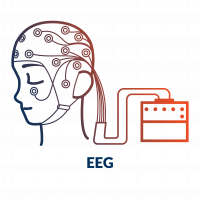
\includegraphics[width=0.6\linewidth]{figures/EEG.png}
    \caption{Illustration of the EEG method.}
    \label{fig:EEG}
\end{figure}


When a single pyramidal cell is stimulated and reaches its threshold, it generates an action potential. During this process, the synapse receives an excitatory signal, leading to a post-synaptic potential where positively charged ions enter the cell. As a result, a relatively negative charge is induced in the nearby extracellular space, which refers to the fluid-filled space surrounding the neuron. As the action potential travels down the dendrite, it eventually exits the cell membrane at locations further away from the synapse, and these locations are referred to as the "source." Consequently, an outward flow of positive charge prevails, leading to a relatively positive charge in the extracellular space. This spatial configuration creates an external dipole, with a relatively negative charge at the distant part of the dendrite and a positive charge closer to the cell body \cite{bromfield2006introduction}.

Since the electrical potential generated by an individual neuron is far too small to be picked up by the recording electrodes, the EEG measurements primarily reflect the summation of synchronous activity from thousands of pyramidal neurons with similar spatial orientation. Neurons with different geometric alignments cannot be measured as their ions do not align in a way that creates detectable waves. Due to the voltage field gradients decreasing with the square of the distance, detecting activity from deep sources in the brain is more challenging compared to currents closer to the skull \cite{bromfield2006introduction}.


The EEG is typically described in terms of rhythmic activity and transients, which are divided into frequency bands. Frequency bands are often extracted using spectral methods, and most of the cerebral signals observed in the scalp EEG fall within the range of 1–20 Hz. Abnormal activity can broadly be classified into epileptiform and non-epileptiform activity. Epileptiform activity is characteristic of people with epilepsy and includes spikes, sharp waves, and spike-wave complexes. In this context, spikes refer to hypersynchronized bursts from a sufficient number of neurons, arising from high-frequency bursts of action potentials. Generalized epileptiform discharges often exhibit an anterior maximum, seen synchronously throughout the entire brain, strongly suggestive of a generalized epilepsy \cite{bromfield2006introduction}.

Detecting and localizing abnormal electrical patterns in EEG represents an important research pursuit. One of the fundamental aspects in this field is the \emph{EEG inverse problem}, which aims to ascertain the spatial distribution of brain activity using potential measures acquired from scalp EEG recordings. In the upcoming section, we will explore the concept of the EEG inverse problem in greater detail and examine its implications for source localization.

\section{The Inverse Problem and Source Localization}
In the field of neuroscience, the inverse problem involves deducing the underlying parameters responsible for a set of measured EEG data. In contrast to the \emph{forward problem}, where known parameters are used to predict the resulting EEG potential, the inverse problem lacks a unique solution. This implies that different configurations of neural sources can produce the same EEG activity distribution on the scalp \cite{hecker2021convdip}.
\rednote{Is it then possible to reach a loss equal to 0?}

The forward problem entails mathematically modeling the relationship between neural current sources in the brain and the resulting EEG measurements on the scalp. This can be described as:

\begin{equation}
\Phi(t) = L \cdot J(t)
\label{eq:forward_problem}
\end{equation}

Here, $\Phi$ represents the vector of measured EEG signals at time $t$, $J(t)$ is the vector of unknown neural current sources at time $t$, and $L$ is the lead field matrix that connects scalp electrode recordings with neural sources. While the full details of the lead field matrix will be explored later, for now, envision it as a geometric arrangement linking the sensitivity of EEG measurements from diverse scalp locations to potential neural current sources within the brain.

Turning our attention to the inverse problem, its essence lies in estimating neural current sources in the brain using measured EEG data—essentially, the reverse of the forward problem. This relationship can be formulated as:

\begin{equation}
J(t) = L^{-1} \cdot \Phi(t)
\label{eq:inverse_problem}
\end{equation}

where, $L^{-1}$ denotes the inverse of the lead field matrix.

However, unlike the forward problem, the inverse problem lacks a unique solution due to its ill-posed nature. As a result, localizing the precise neural sources generating EEG signals becomes a demanding and statistically-driven endeavor. To address the complexities arising from numerous unknowns, techniques such as machine learning and neural networks are employed. Neural networks are designed to narrow down potential solutions, facilitating a more robust and meaningful estimation of the neural sources underlying the measured EEG data.

%In order to understand the underlaying mechanims of the brain and corresponding EEG recordings, biophysically detailed tools are essential. By accurately simulating EEG data, non-linear optimization algorithms such as machine learning algortihms and neural networks can be utialized for solving the EEG inverse problem.

Before embarking on the utilization of neural networks to solve inverse problems, a substantial amount of appropriate EEG data is essential. This data can be obtained through simulated EEG data generated by \emph{forward modeling}. Forward modeling deals with solving the forward problem, \ref{eq:forward_problem} and describes how the electrical activity in various regions of the human cortex gives rise to EEG signals recorded at the scalp electrodes. This process involves the utialization of \emph{head models} that account for the conductivity of different tissues and the geometry of the head. These head models guide the simulation process, aiding in approximating the real-world EEG recordings.


\section{Head Models}
To accurately simulate EEG data and facilitate source localization, the utilization of head models that precisely represent the conductivity distribution within the human head is paramount. Head models serve as computational representations of the anatomical structure of the head, encompassing the brain, skull, cerebrospinal fluid, and scalp. They play a pivotal role in the simulation of how electrical signals originating from current dipoles propagate through diverse tissue compartments, influencing the recorded values at EEG electrodes.

EEG signals are significantly influenced by the biophysical intricacies of the head. Notably, the cerebrospinal fluid exhibits a conductivity of approximately 1.7 S/m, while the skull and scalp possess conductivities of about 0.01 S/m and 0.5 S/m, respectively. These conductivity disparities underscore the necessity for comprehensive head models that consider such variations. Beyond conductivity, these models also account for the influence of tissue arrangement on EEG signals, such as whether a neuronal population resides within a \emph{sulcus} or a \emph{gyrus} \cite{naess2021biophysically}. By employing such a biophysically detailed head model, one can more accurately simulate the impact of various tissues on the distribution of extracellular potential. As a result, this model offers a heightened level of precision in representing EEG signals, leading to improved accuracy in EEG source localization solutions.

\subsection{The New York Head}
The New York Head (NYH) model, developed by the Biomedical Engineering Department in New York, exemplifies a highly detailed computer model tailored for simulating brain electrical activity, with an emphasis on EEG source localization. Grounded in high-resolution anatomical MRI data from 152 adult heads, this model allows the segmentation of six distinct tissue types within the head: scalp, skull, cerebrospinal fluid, gray matter, white matter, and air cavities. Its high level of detail and accuracy makes it an excellent tool for simulating and comprehending brain activity in a realistic manner.

By presenting a three-dimensional representation of the head and brain, coupled with precise information about tissue geometry and electrical properties, the NYH model proves instrumental in investigating brain functions, particularly within the context of EEG measurements and source localization.

For EEG simulations, the NYH model is solved for 231 specific positions representing recording electrodes on the scalp. To predict the EEG signals recorded at different scalp locations, the model utilizes a mathematical representation called the \emph{lead field matrix}. This matrix captures the relationship between the electrical activity in the brain and the electrical potentials recorded on the scalp.

The lead field matrix is essential for linking brain current density to the EEG signals recorded on the scalp. It relies on the reciprocity theorem, which connects brain current caused by an injected current between stimulating electrodes to the potentials picked up by recording electrodes. Specifically, for a fixed pair of stimulating electrodes, the lead field vectors are calculated throughout the head to determine the orientation of the dipole source that generates the largest potential difference between the electrodes. Represented by the symbol $\boldsymbol{L}$, the lead field matrix then establishes the relationship between the brain's current dipole moment and the resulting EEG signals. Mathematically, the lead field matrix $\boldsymbol{L}$ is given by:

\begin{equation}
L = \frac{E}{I},
\label{eq:R2}
\end{equation}

where $I$ denotew the injected current at the electrode locations, and $E$ corresponds to the resulting electric field in the brain \cite{naess2021biophysically}. This equation provides the precise link between the current dipole moment $p$ in the brain and the recorded EEG signals $\Phi$:

\begin{equation}
\Phi = L \cdot p,
\label{eq:EEG_signal}
\end{equation}
\rednote{Is $p$ here the same as J(t) in earlier equation?}

In practical terms, when an injected current of 1 mA flows through the brain, it generates an electric potential $E$ measured in V/m. Thus, a current dipole moment $\textbf{p}$ in the unit of mAm results in EEG signals measured in the unit of V.

For further comprehensive details about the New York Head model, we refer readers to the article: https://www.parralab.org/nyhead/HauHuaPar-embc-2015.pdf.


\section{The Current Dipole Approximation}
By accurately simulating EEG data, non-linear optimization algorithms such as machine learning algortihms and neural networks can be utialized for solving the EEG inverse problem. However, the simulation of intricate neuronal dynamics is a computationally expensive and complex task. An approximation that address this challange and simplifies the simulation phase is the \emph{current dipole approximation}. This approximation is rooted in the observation that the neuron's contribution to the extracellular potential $V_e$ becomes increasingly more dipole-like with an increasing distance.

\rednote{Find other sources than wikipedia}
The key insight behind the current dipole approximation lies in the \emph{multipole expansion}, a technique that comes to our aid when the recording point is situated at a significant distance from the source distribution. While electrical charges, in the context of neural tissue, can lead to the creation of current multipoles, the multipole expansion theorem provides a way to express the extracellular potential $V_e(R)$ in terms of various contributions, where it in the case of EEG signaling becomes apparant that $V_e(R)$ can be approximated by a single dipole.

Neuronal multipoles depend on the spatial arrangement and symmetry of the charge distribution and result from the interplay of current sources and sinks \cite{wiki:multipoles}. The expression for the extracellular potential associated with different multipole orders may take complicated forms, and be hard to interpreted. However, when the distance $R$ from the center of the volume to the recording point surpasses the distance from the volume center to the outermost source, the applicability of multipole expansion becomes evident \cite{jackson1999classical}. Such expansions are namly often beneficial as usually only the first few terms are needed in order to provide an accurate approximation of the original funtion, as we will se now. This representation of the extracellular potential $\phi(R)$ takes the form:

\begin{equation}
  V(R) = \frac{C_{\text{monopole}}}{R} + \frac{C_{\text{dipole}}}{R^2} + \frac{C_{\text{quadrupole}}}{R^3} + \frac{C_{\text{octopole}}}{R^4} + ... .
\label{eq:extracellular_potential}
\end{equation}

where the numerators represents the contributions to the extracellular potential. The terms denoted $C_\text{monopole}$, $C_\text{dipole}$ and $C_\text{quadrupole}$ represents contributions to the extracellulat potential, $V_e$, and can in general be extremely complicated as they depend on the relationship between radial coordinates and symmetry of the current source and measurement electrode. Interestingly, the contributions beyond the dipole term decay more rapidly with distance $R$. This means that in scenarios where we are considerably distant from the source distribution the higher-order terms become negligible, leaving us primarily with the dipole contribution.

This brings us to another interesting observation: The monopole contribution vanishes, stemming from the fact that the net sum of currents over a neuronal membrane is invariably zero. As a consequence, the monopole term dissipates, leaving us with an approximation of the extracellular potential, $V_e$, that relies solely on the dipole contribution:

\begin{equation}
V_e(\textbf{r}) \approx \frac{C_{\text{dipole}}}{R^2} = \frac{1}{4\pi\sigma}\frac{|\textbf{p}| cos \theta}{\lvert\textbf{r}-\textbf{r}_p\rvert^2}.
\label{eq:extracellular_potential_approximation}
\end{equation}

where we have substituded for $C_\text{dipole}$ in terms of other properties. Here $\textbf{p}$ symbolizes the current dipole moment within a medium of conductivity $\sigma$. The distance between the current dipole moment at $\textbf{r}_p$ and the electrode location $\textbf{r}$ is denoted as $R = |\textbf{R}| = |\textbf{r} - \textbf{r}_p|$. Additionally, $\theta$ signifies the angle between $\textbf{p}$ and $\textbf{R}$. This equation is recognized as the dipole approximation and stands as a reliable method for calculating the extracellular potential, particularly when the distance $R$ significantly surpasses the dipole length $d=|\textbf{d}|$. This condition is frequently satisfied in EEG studies \cite{naess2021biophysically}.

Consequently, we have connected the concept of multipole expansion with the validity of the dipole approximation. Through multipole expansion, we can comprehend the intricate extracellular potential in terms of various contributions, and by carefully considering their behavior, we arrive at the precise dipole approximation.

In Figure \ref{fig:dipole_pattern}, we have provided a simulation of the extracellular potential generated by a neuron in response to a single synaptic input, where the spatial distribution of membrane current was explicitly taken into consideration. The Figure has been collected from work done by Torbjørn Næss and Gaute Einevoll. This simulation aligns with the dipole approximation, as it vizualises apparent that the distribution of electric charge in the extracellular potential of the neurons surroundings exhibits distinct dipole patterns when observed from a greater distance. WTFWTF

\begin{figure}
    \centering
    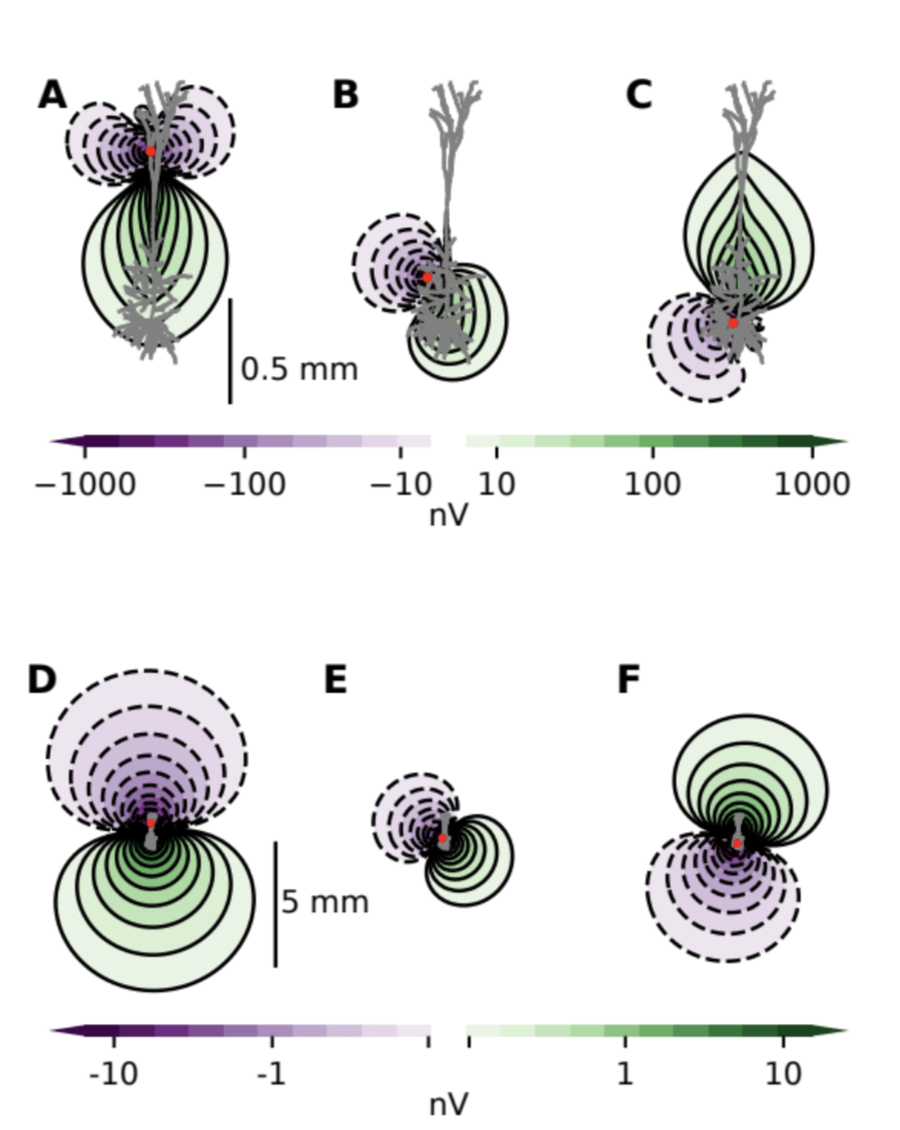
\includegraphics[width=\linewidth]{figures/dipole_pattern.png}
    \caption{Simulation of extracellulat potential showing distinct dipole pattern. The figure has been provided from my supervisiors Torbjørn Ness and Gaute Einevoll.}
    \label{fig:dipole_pattern}
\end{figure}

\section{Solving the EEG inverse problem}
\rednote{Can LFPy fit here or should it be in next chapter?}

In this chapter, we have explored the foundational concepts that underpin the resolution of the inverse problem in EEG source localization. With this groundwork in place, we now turn our attention to the subsequent chapters, where we transition from theory to application.

In the next chapter, we delve into practical implementation by simulating EEG data. Utilizing the New York Head and current dipole approximation, we create synthetic EEG data that closely resembles real-world scenarios. This simulated data, generated using the principles discussed in this chapter, serves as a crucial foundation for the subsequent chapters. It brings us a step closer to addressing the intricate EEG source localization challenge.

Chapter 4 propels us into the realm of machine learning and neural networks. Building upon the simulated EEG data, we construct a sophisticated neural network designed to address the inverse problem efficiently. By harnessing computational techniques, our aim is to bridge the gap between theoretical understanding and real-world applications.


\end{document}